\subsection{Zeitabhängigkeit der Amplitude(Aufgabe a)}
Der Thermodruck mit der eingezeichneten einhüllenden Funktion der abklingenden Amplituden ist in Abbildung \ref{fig:amp} zu sehen.
\begin{figure}[h!]
  \centering
  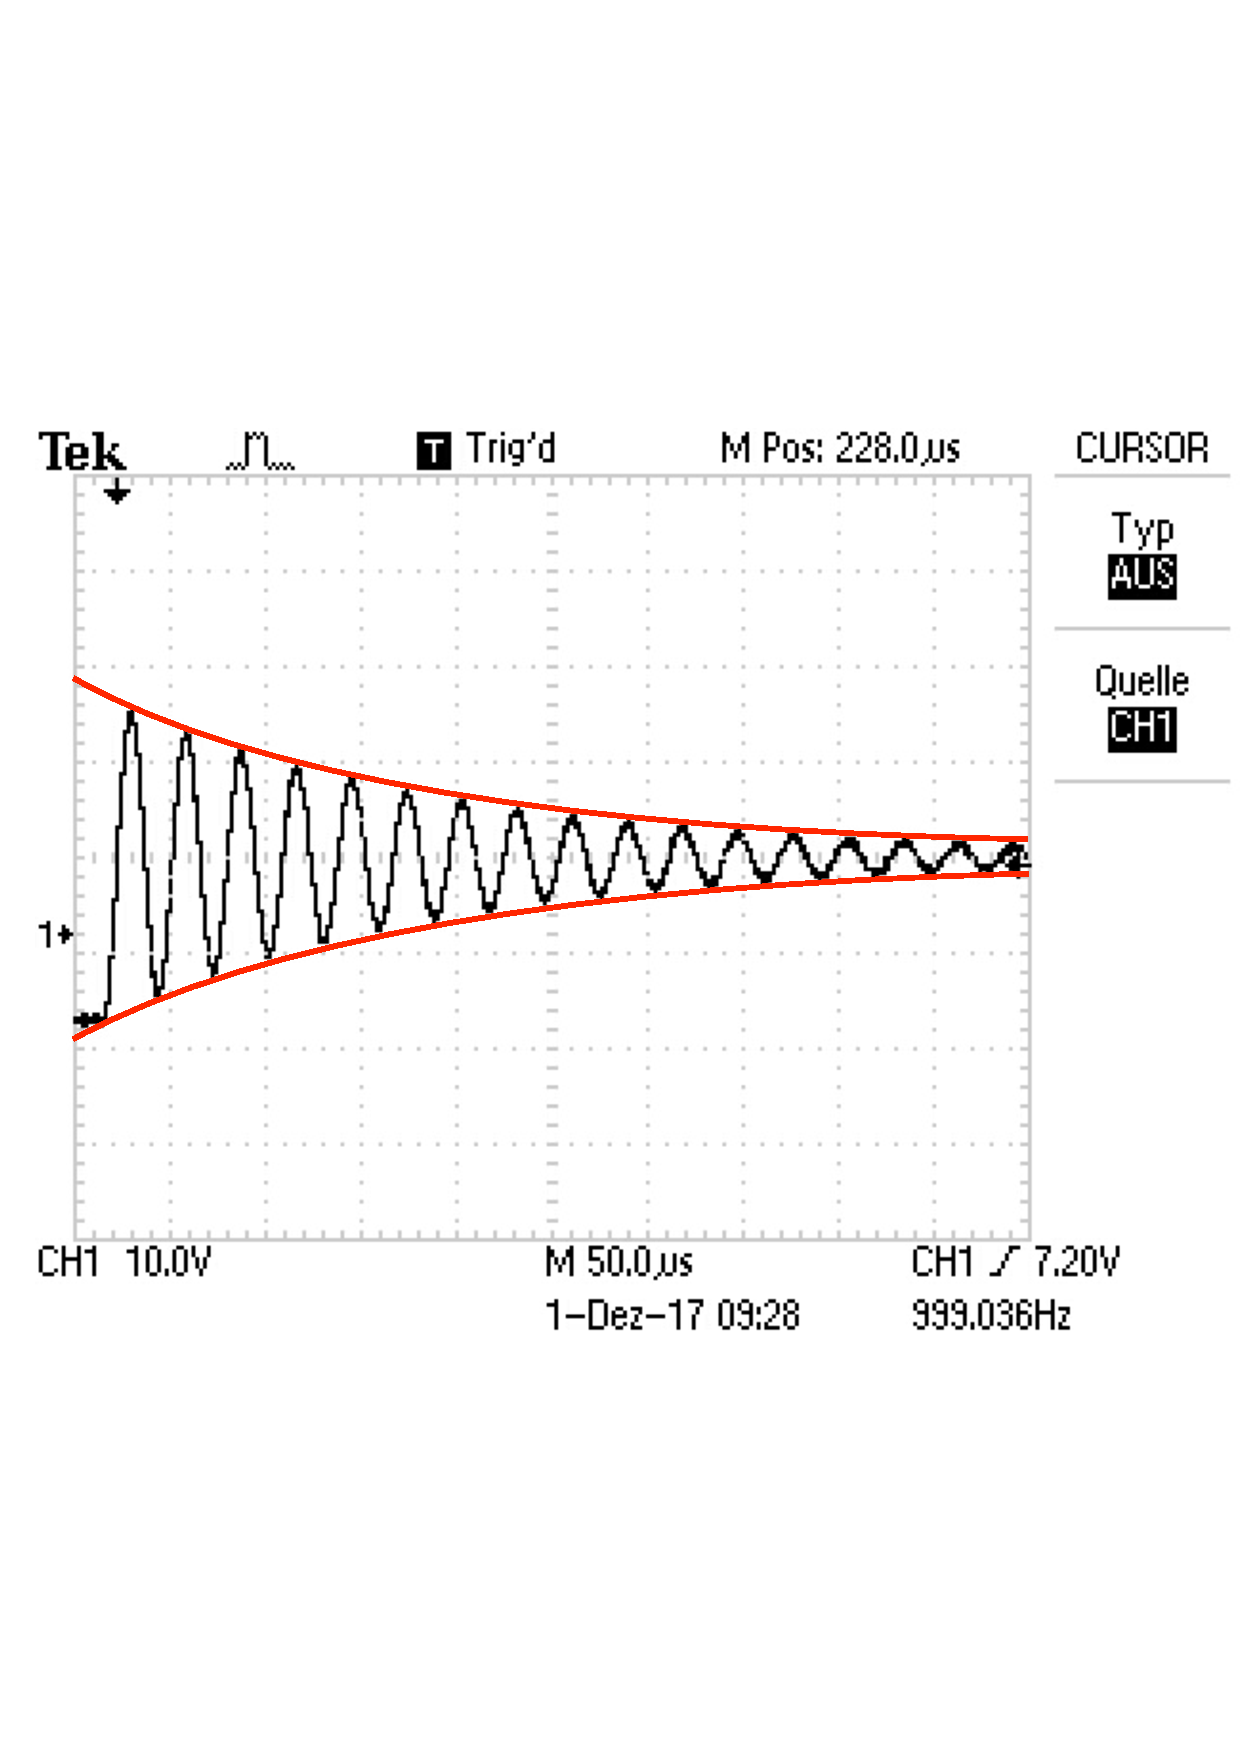
\includegraphics[width=\textwidth]{amp.pdf}
  \caption{Thermodruck mit der einhüllenden Funktion}
  \label{fig:amp}
\end{figure}
Die gemessenen Minima und Maxima sind in Tabelle \ref{tab:amp} eingetragen.
\begin{table}[h!]
  \centering
  \caption{Messdaten: Minima und Maxima der Amplitude}
  \label{tab:amp}
  \begin{tabular}{c c c c}
    \toprule
    U/V & t/$10^{-6}s$ & U/V & t/$10^{-6}s$\\
    \midrule
    -17,2	& -12  &  -8	  & 108 \\
    14,4	& 8    &  8	    & 122 \\
    -14,4	& 22   &  -7,2	& 138 \\
    13,2	& 36   &  6,8 	& 152 \\
    -12	  & 50   &  -6	  & 166 \\
    10,8	& 64   &  6   	& 180 \\
    -10,4	& 80   &  -5,2	& 196 \\
    8,8	  & 94   &  -     &  -  \\
    \bottomrule
  \end{tabular}
\end{table}

Für die Ausgleichsrechnung werden die Beträge der Messwerte verwendet.
Die exponentielle Ausgleichsrechnung in Abbildung \ref{fig:ampfit} mit der Funktion
\begin{equation*}
  A=A_{0} \cdot e^{-2 \pi \mu t}
\end{equation*}
mittels Python ergibt
\begin{align*}
  A_{0} &= \SI{ 15.845 \pm 0.038}{V} \\
    \mu &= \SI{910.581 \pm 672.139}{\frac{1}{s}}.
\end{align*}
\begin{figure}[h!]
  \centering
  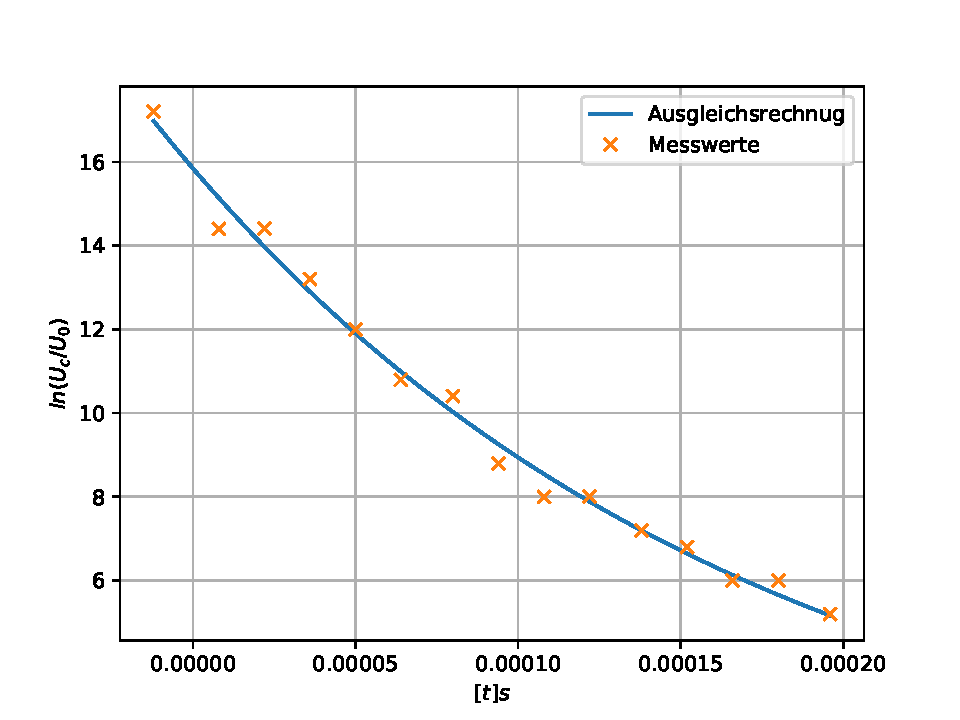
\includegraphics[width=\textwidth]{ampfit.pdf}
  \caption{Exponentielle Regression der Amplitude}
  \label{fig:ampfit}
\end{figure}
\FloatBarrier
Mit Formel \eqref{eqn:mu} wird der effektive Widerstand ermittelt.
Der Fehler ergibt sich über eine Gauß'sche Fehlerfortpflanzung.
\begin{equation*}
  \Delta R_{eff} = \sqrt{ \left( \frac{d R_{eff}}{dL} \right)^2 \cdot (\Delta L)^2 + \left( \frac{d R_{eff}}{d \mu} \right)^2 \cdot (\Delta \mu)^2 }
\end{equation*}
Damit ist der experimentelle effektive Dämpfungswiderstand
\begin{equation*}
  R_{eff}= \SI{115.686 \pm 85.393}{\symup{\Omega}}.
\end{equation*}
Der theoretische Wert des effektiven Dämpfungswiderstands kann nicht genau bestimmt werden, da der Innenwiderstand des Oszilloskops nicht bekannt ist.
Die Abklingdauer wird über Formel \eqref{eqn:tex} berechnet.
Der zugehörige Fehler wird mit der Gauß'schen Fehlerfortpflanzung errechnet:
\begin{equation*}
  \Delta T_{ex, ex} = \sqrt{ \left( \frac{d T_{ex}}{d \mu} \right)^2 \cdot (\Delta \mu)^2 }
\end{equation*}
Somit wird die experimentelle Abklingdauer als
\begin{equation*}
  T_{ex, ex}= \SI{0.00017 \pm 0.00013}{s}
\end{equation*}
bestimmt.
Der theoretische Wert der Abklingdauer errechnet sich über Formel \eqref{eqn:tex}.
Der Fehler errechnet sich über die Gauß'sche Fehlerfortpflanzung
\begin{equation*}
  \Delta T_{ex, theo}= \sqrt{ \left( \frac{d T_{ex}}{dL} \right)^2 \cdot (\Delta L)^2 + \left( \frac{d T_{ex}}{dR} \right)^2 \cdot (\Delta R)^2}
\end{equation*}
Der theoretische Wert der Abklingdauer beläuft sich somit zu
\begin{equation*}
  T_{ex, theo}= \SI{0.0004204 \pm 0.0000015e-7}{s}.
\end{equation*}
\FloatBarrier
\subsection{Bestimmung des Dämpfungswiderstands (Aufgabe b)}
Der Dämpfungswiderstand bei dem aperiodischen Grenzfall wird als
\begin{equation*}
  R_{ap, ex}= \SI{3470}{\symup{\Omega}}
\end{equation*}
gemessen.
Der theoretische Wert des Dämpfungswiderstandes wird mit Formel \eqref{eqn:rap} errechnet.
Der Fehler berechnet sich über die Gauß'sche Fehlerfortpflanzung:
\begin{equation*}
  \Delta R_{ap, theo} = \sqrt{ \left( \frac{d R_{ap}}{dL} \right)^2 \cdot (\Delta L)^2 + \left( \frac{d R_{ap}}{dC} \right)^2 \cdot (\Delta C)^2}
\end{equation*}
So ergibt sich der theoretische Dämpfungswiderstand
\begin{equation*}
  R_{ap, theo} = \SI{4390.387 \pm 9.047}{\symup{\Omega}}.
\end{equation*}

\subsection{Frequenzabhängigkeit der Kondensatorspannung (Aufgabe c)}
Die gemessene Kondensatorspannung und die Frequenz sind in Tabelle \ref{tab:nukond} notiert.

\begin{table}[h!]
  \centering
  \caption{Messdaten: Frequenzabhängigkeit der Kondensatorspannung}
  \label{tab:nukond}
  \begin{tabular}{c c c c c c}
    \toprule
$U_{C}$/V & $\frac{U_C}{U}$ & $\nu$/Hz   &  $U_{C}$/V & $\frac{U_C}{U}$ & $\nu$/Hz\\
    \midrule
  10		&  1,25	  & 15000   &    78		  &  9,75 	 & 36000  \\
  12		&  1,5	  & 20000   &    52		  &  6,5	   & 37000  \\
  16,8	&	 2,1	  & 25000   &    36,8	  &	 4,6	   & 38000  \\
  32		&  4	    & 30000   &    28,8	  &	 3,6	   & 39000  \\
  42		&  5,25 	& 31000   &    23,2	  &	 2,9	   & 40000  \\
  54		&  6,75 	& 32000   &    11,2	  &	 1,4	   & 45000  \\
  82		&  10,25	& 33000   &    7		  &  0,875	 & 50000  \\
  138		&  17,25	& 34000   &    5		  &  0,625	 & 55000  \\
  130		&  16,25	& 35000   &    3,6		&  0,45	   & 60000  \\
    \bottomrule
  \end{tabular}
\end{table}

Die gemessene Erregerspannung $U_{0}$ beträgt dabei $U_{0}=84V$.
$U_{C}/U_{0}$ wird in Abbildung \ref{eqn:res} gegen die Frequenz aufgetragen.
\begin{figure}[h!]
  \centering
  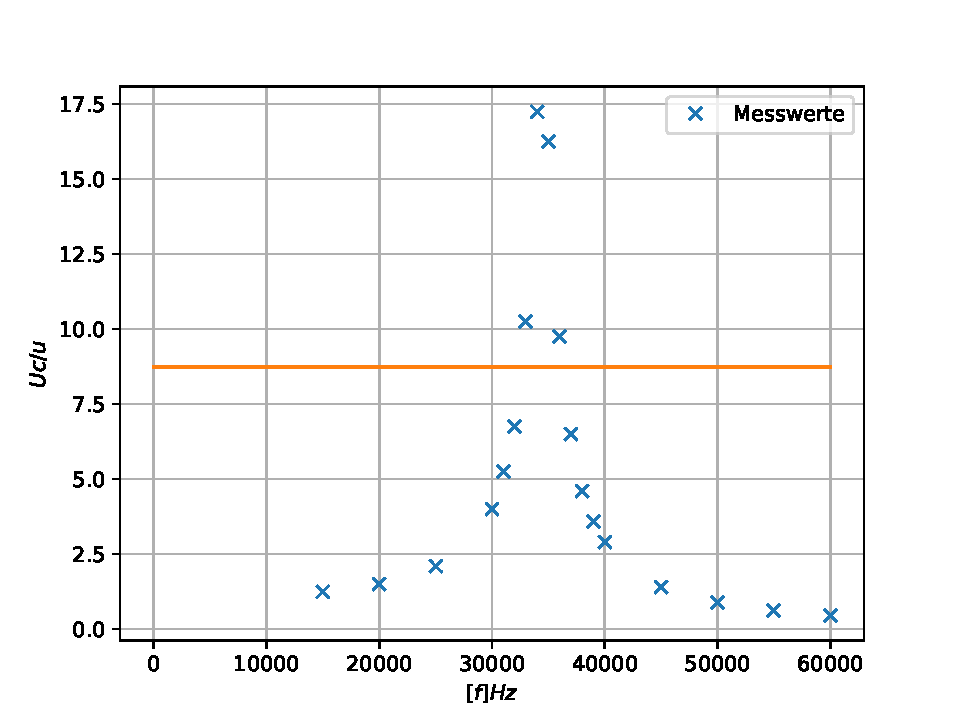
\includegraphics[width=\textwidth]{normkonspan.pdf}
  \caption{Resonanzkurve}
  \label{fig:res}
\end{figure}
Die experimentelle Resonanzüberhöhung wird aus der Abbildung als
\begin{equation*}
  q_{ex} = 17,5
\end{equation*}
abgelesen.
Der theoretische Wert der Resonanzüberhöhung berechnet sich über Formel \eqref{eqn:q}.
Der Fehler wird über die Gauß'sche Fehlerfortpflanzung berechnet:
\begin{equation*}
  \Delta q_{theo} = \sqrt{ \left( \frac{dq}{dR} \right)^2 \cdot (\Delta R)^2 + \left( \frac{dq}{dL} \right)^2 \cdot (\Delta L)^2 + \left( \frac{dq}{dC} \right)^2 \cdot (\Delta C)^2}
\end{equation*}
Die Resonanzüberhöhung ergibt sich zu
\begin{equation*}
  q_{theo}= \SI{45.638 \pm 0.134}.
\end{equation*}
Der experimentelle Wert der Halbwertsbreite b wird aus der Abbildung als
\begin{equation*}
  b_{ex} = \omega_{+} - \omega_{-} = \SI{36428.571}{\frac{1}{s}}
\end{equation*}
abgelesen.
Die theoretische Halbwertsbreite wird durch die Formel \eqref{eqn:halbwertsbreiten} errechnet.
Der Fehler wird über die Gauß'sche Fehlerfortpflanzung ermittelt:
\begin{equation*}
  \Delta b_{theo} = \sqrt{ \left( \frac{db}{dR} \right)^2 \cdot (\Delta R)^2 + \left( \frac{db}{dL} \right)^2 \cdot (\Delta L)^2}.
\end{equation*}
Somit ist der theoretische Wert der Halbwertsbreite
\begin{equation*}
  b_{theo}= \SI{47576.66 \pm 172.34}{\frac{1}{s}}.
\end{equation*}
\FloatBarrier


\subsection{Frequenzabhängigkeit der Phasenverschiebung (Aufgabe d)}
In der Tabelle \ref{tab:Phasen} werden alle wichtigen Messgrößen zur bestimmung von der Resonanzfrequenz $\nu_{res}$ aufgeführt. Desweiteren lässt sich $\nu_1$ und $\nu_2$ für die Phase $\frac {\pi}{4}$ und $\frac{3\pi}{4}$ bestimmen.
In der Graphik \ref{fig:Phasen} wird die Phase gegen die Frequenz aufgetragen.
Mit der Formel \eqref{eqn:nuresonanz} wird $\nu_{res}$ bestimmt. $\nu_1$ und $\nu_{2}$ werden nach Formel \eqref{eqn:phasenverschiebung} berrechnet und mir den abgelesenen werten verglichen.

\begin{align*}
  \nu_{res, exp}  &=& \SI{34e03}{Hz}\\
  \nu_{res, theo} &=& \SI{34,1e03}{Hz}\\
  \nu_{1, exp}    &=& \SI{36,5e03}{Hz}\\
  \nu_{1, theo}   &=& \SI{34,36\pm5,24e03}{Hz}\\
  \nu_{2, exp}    &=& \SI{32,50e03}{Hz}\\
  \nu_{2, theo}   &=& \SI{33,88\pm5,02e03}{Hz}\\
\end{align*}

\begin{table}[h!]
  \centering
  \caption{Messdaten: Frequenzabhängigkeit der Phase}
  \label{tab:Phasen}
  \begin{tabular}{c c c c c c}
    \toprule
f/$10^{3}Hz$ & a/$10^{6}s$ & $\phi$/rad  &  f/$10^{3}Hz$ & a/$10^{6}s$ & $\phi$/rad\\
    \midrule
    15000 &	0     & 0,0      &    36000 &	12,8  & 2,8723   \\
    20000 &	0     & 0,0      &    37000 &	13,2  & 3,14169  \\
    25000 &	0     & 0,0      &    38000 &	13,6  & 3,2368   \\
    30000 &	0,8   & 0,1514   &    39000 &	16,4  & 4,0252   \\
    31000 &	1,6   & 0,3103   &    40000 &	16,4  & 4,2231   \\
    32000 &	1,6   & 0,3222   &    45000 &	13,6  & 3,8841   \\
    33000 &	2     & 0,4189   &    50000 &	10,4  & 3,2673   \\
    34000 &	4     & 0,8607   &    55000 &	9,6   & 3,2782   \\
    35000 &	10,8  & 2,3562   &    60000 &	9,2   & 3,4408   \\
    \bottomrule
  \end{tabular}
\end{table}

\begin{figure}[h!]
  \centering
  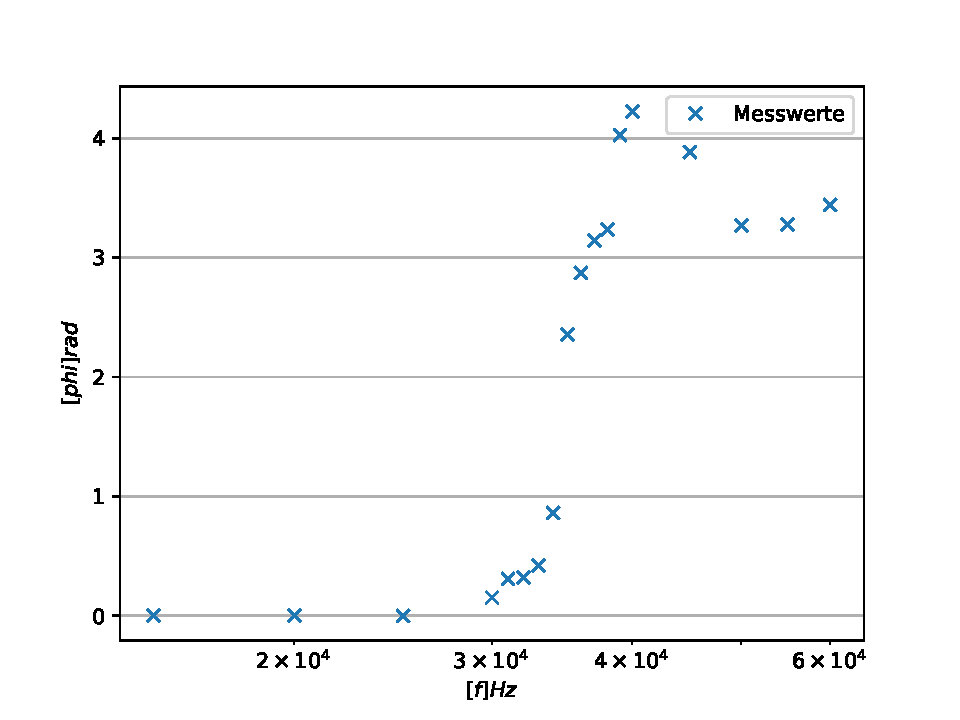
\includegraphics[width=\textwidth]{Phasschib.pdf}
  \caption{Phasenverschiebung}
  \label{fig:Phasen}
\end{figure}
\FloatBarrier
